% ============================================================
% EqWM-FPS: Z2-Equivariant World Models for Imagination Training
% in a First-Person Shooter: Reward-Head Stability without Return Gains
% Submitted to: Neural Networks (Elsevier)
%
% v3 (2026-10-02): response to external review. Identical body to
% eqwm_acmart_v3.tex (acmart preview edition); only the document class
% and front matter differ. To switch to ECAI/UAI: change the
% \documentclass line and the \journalnote below; body is unchanged.
% Changes vs v2 (frozen 2026-10-01 19:29): see eqwm_acmart_v3.tex header.
% ============================================================
\documentclass[preprint,12pt]{elsarticle}
% ECAI/UAI switch: replace the line above with, e.g.,
%   \documentclass[10pt,a4paper]{article}
% and use natbib/icml style; the body is journal-agnostic.

\journal{Neural Networks}

\usepackage{graphicx}
\usepackage{amsmath,amssymb}
\usepackage{booktabs}
\usepackage{multirow}
\usepackage{xcolor}
\usepackage{url}
\usepackage{enumitem}
\graphicspath{{figs/}}

% theorem-like environments
\newtheorem{theorem}{Theorem}
\newtheorem{corollary}[theorem]{Corollary}
\newtheorem{proposition}{Proposition}

\bibliographystyle{elsarticle-num}

\begin{document}

\begin{frontmatter}

\title{Z$_2$-Equivariant World Models for Imagination Training\\
in a First-Person Shooter: Reward-Head Stability without Return Gains}

\author[1]{Anonymous}
\address[1]{Anonymous Institution (double-blind review)}

\begin{abstract}
First-person shooter (FPS) games stress deep reinforcement learning (RL):
visual observations are high-dimensional and sample complexity is
prohibitive. World models cut real-environment interaction by training the
policy inside a learned dynamics model, but most implementations ignore the
left--right mirror symmetry that FPS environments possess almost by
construction. We study \emph{EqWM}, a compact world model and PPO policy that
enforce horizontal-flip ($\mathbb Z_2$) equivariance by group averaging across
encoder, recurrent dynamics, decoder, and reward head, on the ViZDoom
\texttt{health\_gathering} benchmark \cite{vizdoom2016}. We report findings
without inflation; the honest headline is stability rather than returns. The
equivariant reward head is markedly more stable across seeds, with
reward-prediction MAE $0.104\pm0.025$ versus $0.223\pm0.099$, but a
constant-predictor analysis shows the reward is near-degenerate and both
heads barely exceed predicting its mean: the benefit is cross-seed stability
of a task-relevant but not well-learned head, not evidence of reward
understanding. Single-frame reconstruction is statistically indistinguishable
and marginally favors the non-equivariant model. Imagination training reaches,
after about $15$k real steps, returns comparable to pure PPO at $20$k--$40$k
steps, an order-of-$2\times$ sample-efficiency gain that we mark as
preliminary, with a measured step ratio of $1.3$--$2.7\times$ and flat noisy
curves. Under this small-model budget, equivariant and non-equivariant
imagination variants are not distinguishable, and a four-cell ablation pooled
over nine same-machine seeds finds no significant return gain, with the fully
equivariant configuration numerically highest but far from significance and
not stably ordered across seed sets. A
bootstrap estimate of the effective-sample multiplier is non-monotone and
cross-machine inconsistent. The theory is presented as upper bounds and an
explicitly qualitative scaling law, with every experimental support, weak
support, or contradiction marked.
\end{abstract}

\begin{keyword}
Equivariant neural networks \sep World models \sep Imagination training \sep Reinforcement learning \sep First-person shooter \sep PAC-Bayes
\end{keyword}

\end{frontmatter}

%% ===================== 1. INTRODUCTION =====================
\section{Introduction}
Deep reinforcement learning (RL) has reached superhuman levels in many
games, but training an agent directly from raw pixels in first-person
shooters (FPS) still demands millions of environment interactions
\cite{fps2017,vizdoom2016}, which is impractical when environment access is
expensive. \emph{World models} address this by learning a predictive model
of the environment and optimizing the policy entirely inside it
\cite{worldmodels2018}. The Dreamer family operationalizes this idea with a
recurrent state-space model \cite{dreamerv1,dreamerv2,dreamerv3} and has
recently scaled to long-horizon tasks inside learned models
\cite{dreamer42025}; model-based planning with a learned dynamics model is
the core of MuZero \cite{muzero2020}, and model-based policy optimization
exploits such models for data efficiency \cite{mbpo2019}.

FPS environments, however, possess a near-perfect structural symmetry that
none of these general-purpose architectures exploit: the rendered scene and
its dynamics are (approximately) invariant under a horizontal flip, and a
flipped camera view should induce flipped actions
(TURN\_LEFT $\leftrightarrow$ TURN\_RIGHT, MOVE\_FORWARD unchanged).
Group-equivariant networks \cite{gcnn2016} bake such symmetries into the
architecture and, in principle, use each observation several times at no extra
data cost. This is precisely the data-starved regime in which world models
operate.

We ask a deliberately narrow question: \emph{on a small FPS benchmark, does
$\mathbb Z_2$ equivariance in the world model and policy improve sample
efficiency or final return, and how should that be measured honestly?} Our
system, \emph{EqWM}, enforces hard equivariance by group averaging
\cite{gcnn2016} at every convolutional layer of the encoder, recurrent
dynamics, decoder, and policy, with an invariant reward head and an
antisymmetric left/right action head. Our contributions are:
\begin{enumerate}[leftmargin=*]
  \item \textbf{Implementation and controlled comparison on ViZDoom.} We
        build an equivariant ConvGRU world model and equivariant PPO policy
        for \texttt{health\_gathering} and compare them against matched
        non-equivariant baselines, reporting per-seed, aggregated, and
        pooled-seed statistics (Section~\ref{sec:exp}).
  \item \textbf{PAC-Bayes-style analysis of imagination training.} We state
        three results: a world-model prediction bound that depends on an
        effective sample count $N_{\rm eff}$ (Theorem~\ref{th:wm}), an
        imagination-training generalization bound that separates world-model
        bias from estimation error (Theorem~\ref{th:imag}), and a scaling law
        for the optimal real-to-imagination ratio
        (Corollary~\ref{cor:ratio}); proofs are given in
        Appendix~\ref{app:proofs}, and a bootstrap estimator with an explicit
        bias-variance caveat (Proposition~\ref{prop:meff}) is provided.
  \item \textbf{Honest empirical verdict.} The clearest measured benefit of
        equivariance is \emph{cross-seed stability of the reward head}, which
        a constant-predictor analysis shows to be stability of a
        near-degenerate predictor rather than evidence of reward
        understanding; imagination training gives an order-of-$2\times$
        sample-efficiency gain over pure PPO that is preliminary; a four-cell
        ablation pooled over nine same-machine seeds shows no significant
        return gain from any equivariant component; and the bootstrap estimate
        of the effective-sample multiplier is not robust. We treat the weak
        and negative results as limitations and open problems rather than
        burying them.
\end{enumerate}

The remainder of the paper is organized as follows. Section~\ref{sec:rw}
reviews related work. Section~\ref{sec:prelim} fixes notation.
Section~\ref{sec:method} details the architecture. Section~\ref{sec:theory}
states the theory. Section~\ref{sec:exp} reports experiments, and
Section~\ref{sec:concl} concludes with limitations.

%% ===================== 2. RELATED WORK =====================
\section{Related Work}\label{sec:rw}

\paragraph{World models and imagination training.}
Learning a predictive model for RL dates back to Ha and Schmidhuber
\cite{worldmodels2018}. The Dreamer series \cite{dreamerv1,dreamerv2}
operationalized latent imagination with a recurrent state-space model, and
DreamerV3 \cite{dreamerv3} showed a single model can solve many domains; the
most recent Dreamer4 \cite{dreamer42025} scales agent training inside a
fast world model in Minecraft. MuZero \cite{muzero2020} pairs learned
dynamics with planning, and MBPO \cite{mbpo2019} uses an ensemble of models
to cut real samples. Concurrent with these, EMERALD \cite{emerald2025}
improves world modeling with masked latent transformers and strong
sample efficiency on Crafter. Our work follows the Dreamer-style
``train PPO inside a learned latent model'' loop but restricts the model class
to a group-equivariant one.

\paragraph{Equivariant reinforcement learning.}
Group-equivariant convolutions were introduced by Cohen and Welling
\cite{gcnn2016}. In RL, MDP homomorphic networks \cite{mdphomo2020} and group
equivariant deep RL \cite{geodrl2020} encode state/action symmetries, while
$\mathrm{SO}(2)$-equivariant policies \cite{so2rl2022} and group-invariant
representation structuring \cite{groupinv2022} exploit continuous rotation
symmetries. The closest lines to ours are equivariant model-based RL: Park
et al.\ learn symmetric embeddings for equivariant world models
\cite{sen2022}, Deac et al.\ make MuZero equivariant \cite{eqmuzero2023},
and EDGI builds an SE(3)-equivariant diffusion planner for embodied agents
\cite{edgi2023}. Multi-group equivariant augmentation \cite{multigroup2025}
studies several symmetry groups in manipulation. Unlike these works, which
target control, board games, or 3D/SE(3) embodied settings, we target 2D
FPS pixels with the discrete $\mathbb Z_2$ group and integrate equivariance
into \emph{both} the world model and the imagination-training loop, while
reporting the small-benchmark result transparently.

\paragraph{PAC-Bayes and generalization in RL.}
PAC-Bayes bounds \cite{mcallester1999} relate a posterior's risk to its
empirical risk through a KL complexity term. Recent PAC-Bayesian RL
\cite{pacbayesrl2025} trains generalizable on-policy policies. We adapt the
decomposition to the mixed real/imagination data regime and use the bootstrap
\cite{bootstrap1993} to estimate the effective sample multiplier empirically.

\paragraph{FPS reinforcement learning.}
ViZDoom \cite{vizdoom2016} provides a Doom-based visual-RL benchmark; early
agents trained directly with model-free RL \cite{fps2017}. To our knowledge,
prior work has not combined an equivariant world model with imagination
training on FPS pixels.

%% ===================== 3. PRELIMINARIES =====================
\section{Preliminaries}\label{sec:prelim}

\paragraph{MDP.}
We model the environment as an MDP
$\langle\mathcal S,\mathcal A,P,r,\gamma\rangle$ \cite{suttonbarto2018},
where $\mathcal S$ is the RGB frame space,
$\mathcal A=\{\textsc{turn-left},\textsc{turn-right},\textsc{forward}\}$ is a
three-action discrete set, $P$ the transition kernel, $r$ the reward, and
$\gamma=0.99$ the discount. The objective is the expected discounted return
$J(\pi)=\mathbb E_{\pi}[\sum_t\gamma^t r_t]$.

\paragraph{Group action and equivariance.}
We take $G=\mathbb Z_2=\{e,h\}$, where $h$ is a horizontal flip. The group
acts on observations by $h\cdot x=\mathrm{flip}_W(x)$ and on actions by the
permutation $h\cdot\textsc{turn-left}=\textsc{turn-right}$,
$h\cdot\textsc{turn-right}=\textsc{turn-left}$,
$h\cdot\textsc{forward}=\textsc{forward}$. A map $f$ is
\emph{equivariant} if $f(gx)=g f(x)$ and \emph{invariant} if $f(gx)=f(x)$.

\paragraph{World models and imagination.}
A world model $\hat M=\langle\hat P,\hat r\rangle$ approximates the
environment. Given $\hat M$, imagination training starts a policy rollout
from a real observation and predicts subsequent latent states and rewards
with $\hat M$, then updates the policy (here PPO \cite{ppo2017}) on these
imagined trajectories \cite{dreamerv3}.

\paragraph{PAC-Bayes.}
With posterior $\rho$, prior $\pi$, and $n$ i.i.d.\ samples, a canonical
bound is
$R(\rho)\le R_S(\rho)+\sqrt{(\mathrm{KL}(\rho\|\pi)+\log(2\sqrt n/\delta))/(2n)}$.

%% ===================== 4. METHOD =====================
\section{Method}\label{sec:method}

\begin{figure}[t]
  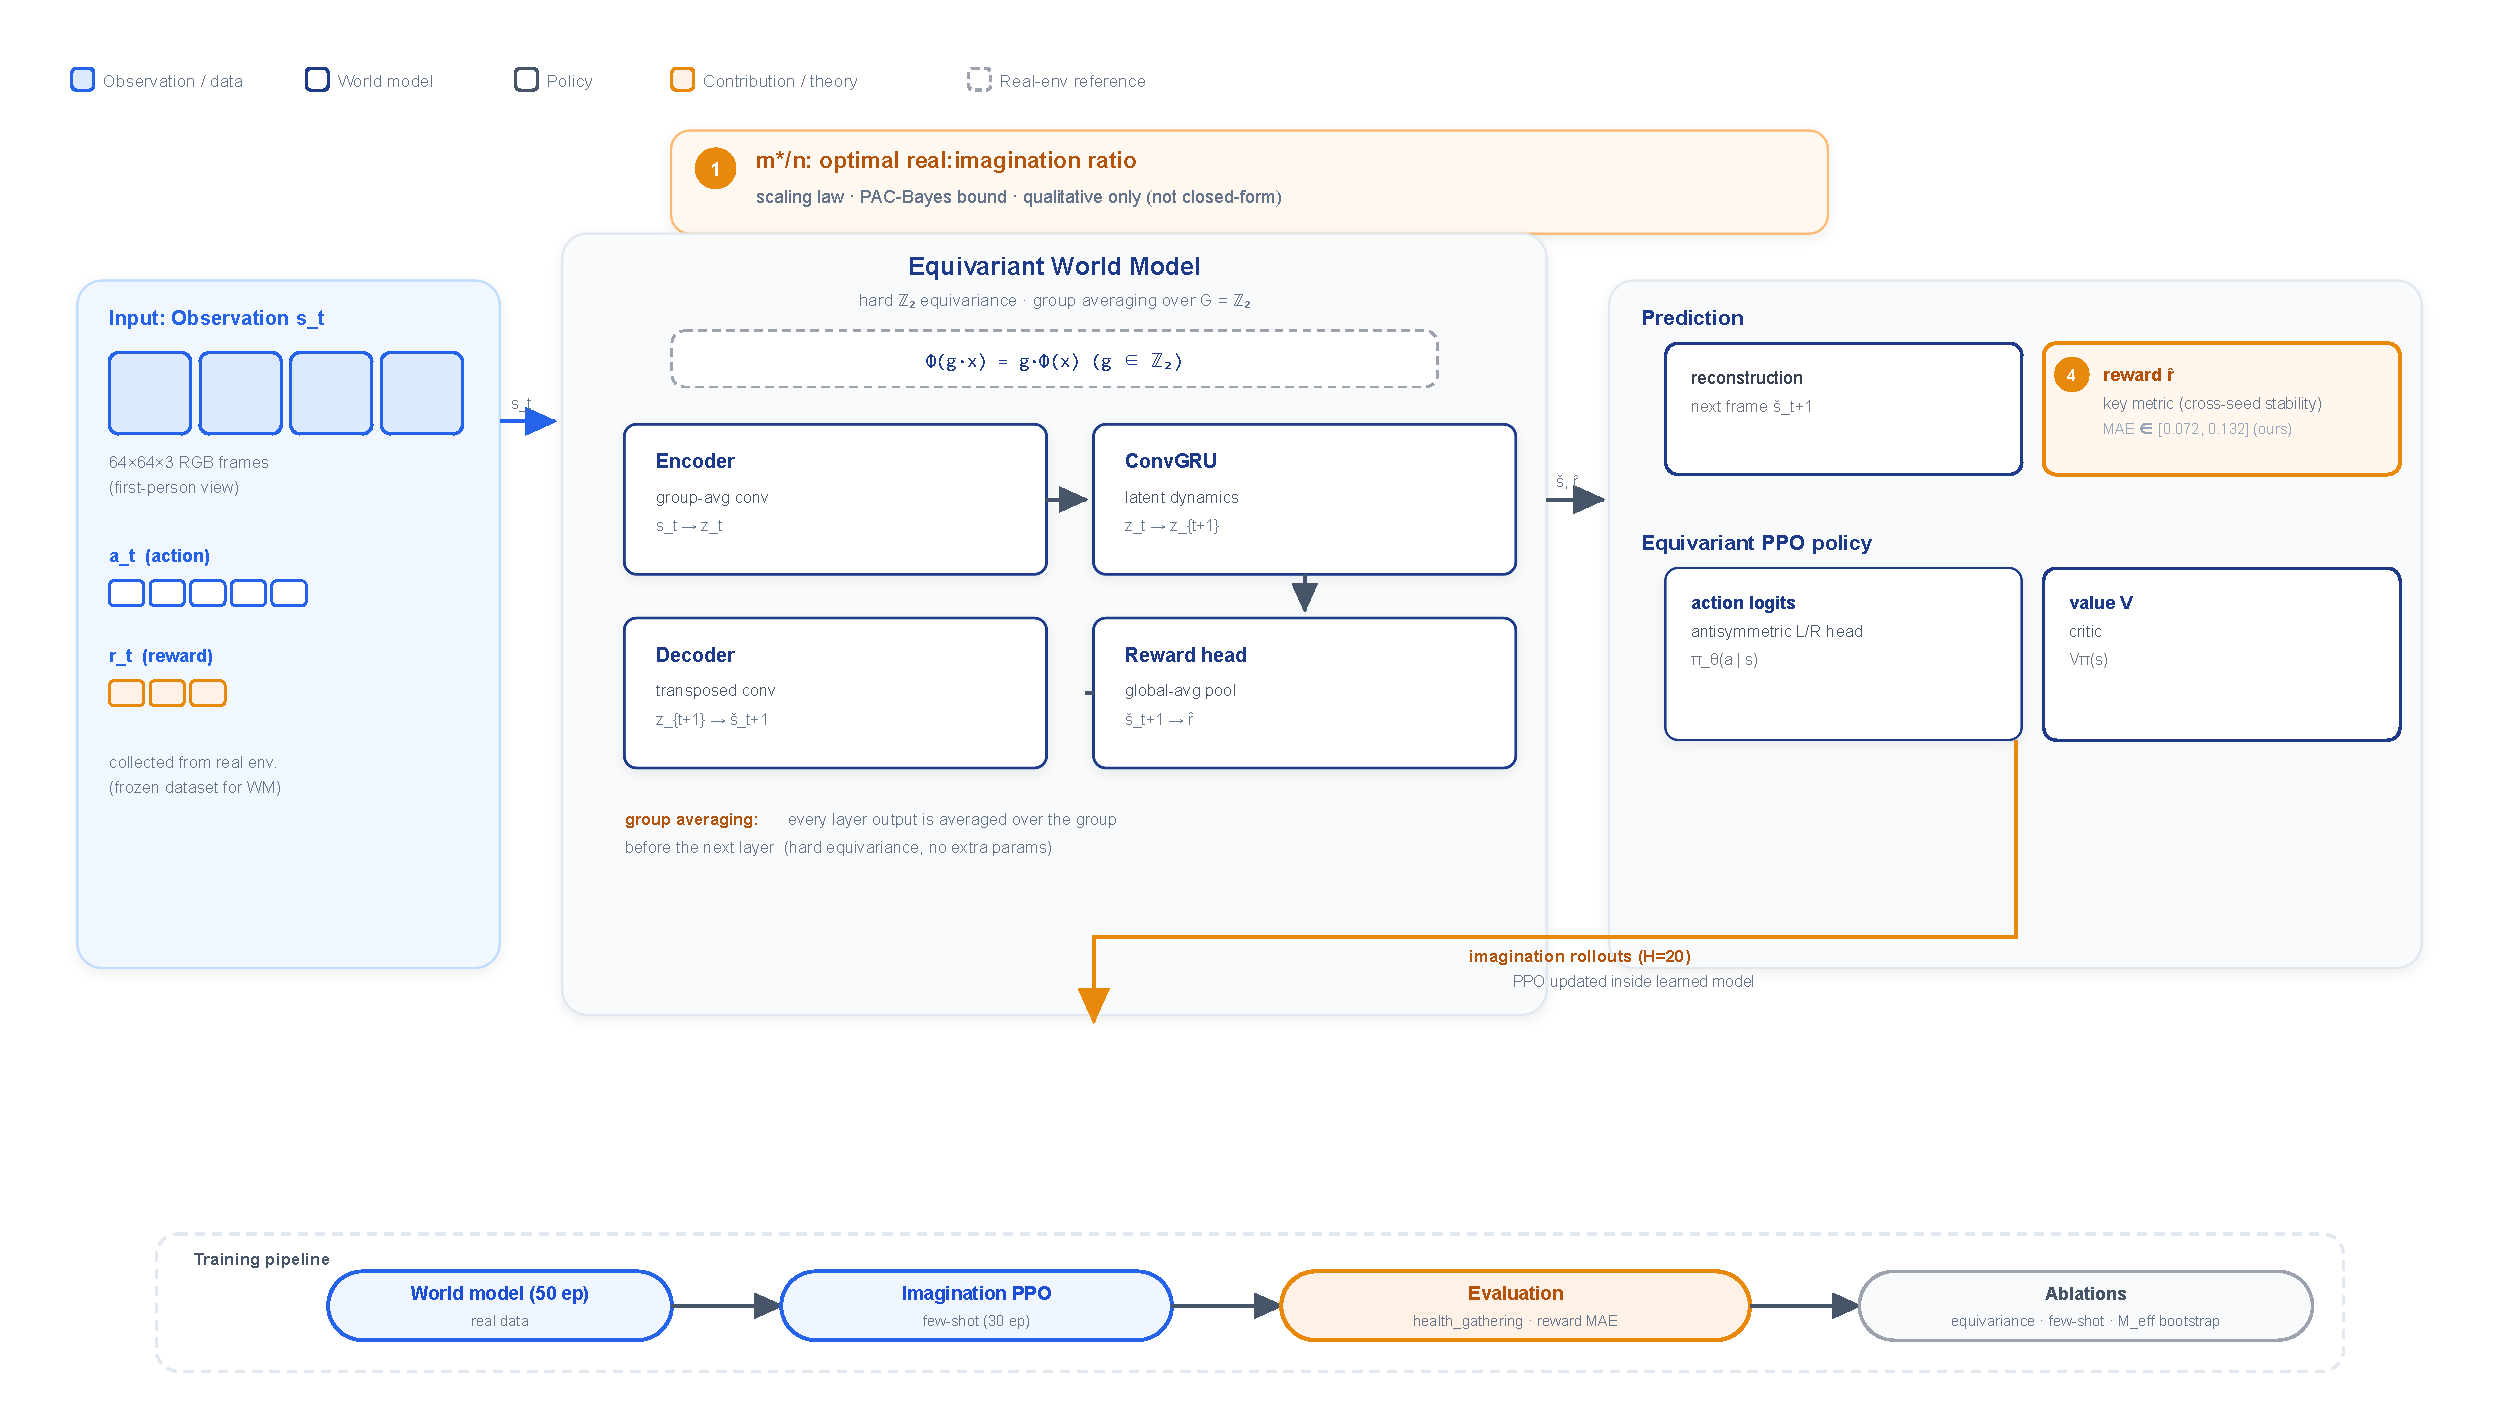
\includegraphics[width=0.9\textwidth]{eqwm_fig1.pdf}
  \caption{Overview of the equivariant world model and imagination training. The world model enforces hard $\mathbb Z_2$ equivariance by group averaging across an Encoder, a ConvGRU dynamics cell, a Decoder, and a reward head; it predicts both frame reconstruction and a scalar reward. The equivariant PPO policy is updated inside the learned model on imagination rollouts, and the analysis bounds the optimal real:imagination ratio $m^*/n$ only qualitatively.}
  \label{fig:overview}
\end{figure}


\subsection{Equivariant $\mathbb Z_2$ world model}
The world model $\hat M_\phi$ has four parts (Figure~\ref{fig:overview}).
\emph{Encoder} $E_\phi$: three strided convolutions map a
$64\times64\times3$ frame to an $8\times8\times z$ latent map
($z=32$, base channels $16$). Every convolution is a group-averaging layer
\cite{gcnn2016},
\begin{equation}
  E_\phi(x)=\tfrac12\big[\mathrm{Conv}(x)+\mathrm{flip}_W(\mathrm{Conv}(\mathrm{flip}_W(x)))\big],
\end{equation}
which shares one kernel and satisfies
$E_\phi(\mathrm{flip}_W x)=\mathrm{flip}_W E_\phi(x)$ up to numerical
precision. \emph{Dynamics}: an equivariant ConvGRU cell updates the latent
map from the previous map and a spatially broadcast one-hot action; gates
use the same group-averaging convolution. \emph{Decoder}: three equivariant
transposed convolutions reconstruct the frame with a sigmoid output.
\emph{Reward head}: a global-average-pooling (invariant) layer followed by an
MLP predicts a scalar reward from the latent map. The non-equivariant
baseline uses identical widths and layer counts but ordinary convolutions, a
flattened encoder for its heads, and no group averaging.

The training loss is reconstruction MSE plus reward MSE plus latent-dynamics
MSE, and (only for the equivariant model) a soft consistency penalty on the
encoder and dynamics under flip.

\subsection{Equivariant PPO policy}
The policy uses the same equivariant encoder. Invariant features
($\mathrm{gap}(h)$) drive the forward action and the (invariant) value head;
an antisymmetric feature $a=\overline{h_{\rm left}}-\overline{h_{\rm right}}$
distinguishes left and right:
$\ell_{\rm left}=s+a$, $\ell_{\rm right}=s-a$, $\ell_{\rm forward}=s'$.
This enforces $\pi(h\cdot x)=h\cdot\pi(x)$.

\subsection{Imagination pipeline}
We collect $n=10$k random real transitions, train $\hat M_\phi$ for 30
epochs, then iterate: collect $1{,}000$ new on-policy real transitions,
fine-tune $\hat M_\phi$ for 5 epochs, imagine short rollouts of horizon
$H=20$ under PPO \cite{ppo2017} (200 rollouts per outer step), and update on
the imagined data. This gives roughly $4{,}000$ imagined transitions per
$1{,}000$ new real transitions, i.e.\ an imagination ratio $\approx4$, fixed
rather than tuned. Table~\ref{tab:hyper} lists all hyper-parameters.

\begin{table}[t]
\centering
\caption{Hyper-parameters (identical for equivariant and standard variants
except for group averaging). Exp.\,1 trained the world model for 50 epochs;
the imagination runs below use 30 initial epochs.}
\label{tab:hyper}
\footnotesize\setlength{\tabcolsep}{3pt}
\begin{tabular}{@{}lll@{}}
\toprule
Group & Hyper-parameter & Value \\
\midrule
Environment & Observation & $64\times64\times3$ RGB, frame skip $4$ \\
            & Discount $\gamma$ & $0.99$ \\
World model & Base channels / latent $z$ & $16$ / $32$ ($8\times8\times32$) \\
            & Init. real steps $n$ & $10{,}000$ \\
            & WM epochs (init / fine-tune) & $30$ / $5$ \\
Imagination & Horizon $H$ & $20$ \\
            & Imagined rollouts / outer step & $200$ \\
            & New real steps / outer step & $1{,}000$ \\
            & Imagination ratio $m/n$ & $\approx4$ \\
PPO         & Optimizer / LR & Adam / $3\times10^{-4}$ \\
            & Minibatch / epochs & $256$ / $4$ \\
            & Clip / GAE $\lambda$ & $0.2$ / $0.95$ \\
            & Entropy / value coef. & $0.01$ / $0.5$ \\
Bootstrap   & Resamples $B$ / train set & $15$ / $8{,}000$ \\
\bottomrule
\end{tabular}
\end{table}

%% ===================== 5. THEORY =====================
\section{Theory}\label{sec:theory}
We present three results and one estimator. They are intentionally stated as
\emph{upper bounds and a qualitative scaling law}; our claim is about the
structure of the trade-off, not tightness. Before the statements we fix a
notation conflict: throughout, $N_{\rm eff}$ is an \emph{effective sample
count} (dimension of data, $\le |G|n$), whereas $R_{\rm boot}$ in
Proposition~\ref{prop:meff} is the \emph{dimensionless variance ratio} we
estimate from data; Proposition~\ref{prop:meff} makes $R_{\rm boot}$ an
empirical proxy for the multiplier $N_{\rm eff}/n$ whose error is not
quantified.

\begin{theorem}[World-model prediction bound]\label{th:wm}
Let $\hat M_\phi$ be trained on $n$ transitions. With probability
$\ge1-\delta$ over the data,
\[
  \mathbb E_{(s,a,s')}\|\hat P_\phi(s,a)-s'\|^2
  \le \hat{\mathcal L}_{\rm WM}(S)+
  O\!\left(\sqrt{\tfrac{\mathrm{KL}(\phi\|\phi_0)+\log(1/\delta)}{N_{\rm eff}}}\right),
\]
where $N_{\rm eff}\le |G|\,n$ is the effective sample count.
\end{theorem}

\paragraph{Proof sketch.}
Start from the standard PAC-Bayes inequality
$R(\phi)\le R_S(\phi)+O(\sqrt{(\mathrm{KL}(\phi\|\phi_0)+\log(1/\delta))/n})$
\cite{mcallester1999}. Because transitions within a rollout are temporally
correlated, group the data into independent blocks and apply McDiarmid's
inequality over blocks; this replaces $n$ by an effective block count. Group
averaging \emph{reuses} each transition together with its flipped copy, so
the independent data effectively available is at most $|G|$ times the raw
count, i.e.\ $N_{\rm eff}\le |G|n$. Note this is a \emph{data-reuse} effect
only: the group-averaging layer shares a single kernel (\S\ref{sec:method})
and does not reduce the parameter count. A full block-decomposition proof is
given in Appendix~\ref{app:proofs}; the bound is order-level and not tuned.

\begin{theorem}[Imagination-training bound]\label{th:imag}
A policy trained on $n$ real and $m$ imagined transitions satisfies, with
probability $\ge1-\delta$,
\[
  J(\pi_\theta)\ge \hat J_{\rm imag}(\pi_\theta)
  -C\,\varepsilon_{\rm WM}\,H
  -O\!\left(\sqrt{\tfrac{\log(1/\delta)}{n+m\eta}}\right),
\]
where $\varepsilon_{\rm WM}$ is the world-model error, $H$ the imagination
horizon, and $\eta\in[0,1]$ down-weights imagined data by model accuracy.
\end{theorem}

\paragraph{Proof sketch.}
The gap splits into two terms. \emph{Model-bias term}: an $H$-step rollout
compounds one-step error geometrically,
$\sum_{t=0}^{H-1}\gamma^t\varepsilon_{\rm WM}\le C\,\varepsilon_{\rm WM}H$
for a constant $C$ that depends on the discount and on the policy's Lipschitz
constant. \emph{Estimation term}: treating imagined transitions as
weight-$\eta$ samples, the effective data count is $n+m\eta$, to which the
PAC-Bayes/McDiarmid estimation bound applies directly. The two terms are
independent and additive; the proof is in Appendix~\ref{app:proofs}.

\begin{corollary}[Optimal real:imagination ratio, as a scaling law]\label{cor:ratio}
Equating the estimation slack of Theorem~\ref{th:imag} to a fixed fraction
of its model-bias slack and solving for $m$ gives the scaling law
\begin{equation}
  \frac{m^*}{n}=C\,\frac{N_{\rm eff}/n}{\varepsilon_{\rm WM}^{2}},
\end{equation}
for a constant $C$ that absorbs the horizon, the discount, the weight
$\eta$, and the (unknown) variance scale.
\end{corollary}

We emphasize that Corollary~\ref{cor:ratio} is a \emph{scaling law}, not a
numerically tight formula: substituting the pixel MSE
$\varepsilon_{\rm WM}\approx10^{-2}$ literally yields $m^*/n=10^4$, which is
unrealistically large because the constant and the units of
$\varepsilon_{\rm WM}$ are uncalibrated. We therefore clip the ratio to a
fixed range in practice and treat the corollary as qualitative guidance,
exactly as Section~\ref{sec:exp} reports. The derivation (Appendix
\ref{app:proofs}) is an order-level argument, not a sharp optimization
result.

\begin{proposition}[Estimating the multiplier by bootstrap]\label{prop:meff}
The multiplier $N_{\rm eff}/n$ can be estimated by bootstrap
\cite{bootstrap1993}: draw $B$ resamples of the training set, refit, and set
\begin{equation}
  R_{\rm boot}=\frac{\widehat{\operatorname{Var}}_{\rm std}}{\widehat{\operatorname{Var}}_{\rm eq}},
  \qquad
  \widehat{N_{\rm eff}/n}=\operatorname{clip}(R_{\rm boot},\,1,\,|G|=2).
\end{equation}
\end{proposition}

\paragraph{Justification and caveats.}
For an i.i.d.\ estimator with $n$ samples, the out-of-sample error variance
scales as $1/n$; if equivariance multiplies the effective data by $k$, its
error variance scales as $1/(kn)$, so the variance ratio recovers $k$. The
bootstrap \cite{bootstrap1993} estimates these two variances by resampling.
The clip to $[1,|G|]$ encodes the prior that a symmetry group of size $|G|$
cannot multiply data by more than $|G|$. Three caveats make $R_{\rm boot}$ an
\emph{empirical proxy with unknown error} rather than an estimator of
$N_{\rm eff}/n$: (i)~the identity $R_{\rm boot}\approx N_{\rm eff}/n$ holds
only when the estimator's error is variance-dominated, whereas model bias
adds a non-vanishing shared term to both variances; (ii)~RL transitions are
temporally correlated, so the resampling assumption is only approximate; and
(iii)~optimization noise (SGD seed) inflates both variances independently.
Section~\ref{sec:exp} therefore treats $R_{\rm boot}>1$ as unconfirmed.

%% ===================== 6. EXPERIMENTS =====================
\section{Experiments}\label{sec:exp}

\subsection{Setup}
We use ViZDoom \texttt{health\_gathering}: the agent navigates a maze to
collect health packs while taking damage; observations are $64\times64\times3$
RGB frames with frame skip $4$. The reward is near-degenerate: the agent is
penalized only at death, so roughly $99.3\%$ of non-terminal steps carry an
identical reward offset (empirically, $99.3\%$ of steps yield $+4$ and
$0.7\%$ yield $-96$, with rewards standardized during world-model training).
This sparsity makes the reward head easy to overfit and motivates the
stability analysis below. The small model (base channels $16$, latent
$8\times8\times32$) is used throughout. We report mean$\pm$std over seeds and
state the seed count explicitly for every number; all reward metrics are in
the standardized reward space used for training.

\subsection{Experiment 1: world-model prediction and reward-head stability}
Both world models are trained on $10$k random transitions for 50 epochs over
three seeds (Table~\ref{tab:wm}).

\begin{table}[t]
\centering
\caption{World-model comparison on \texttt{health\_gathering} (10k steps,
50 epochs, 3 seeds; mean$\pm$std). Reward MAE is in the standardized reward
space. The two constant baselines are reference points, not trained models
(see the reward-head analysis in the text); the earlier concatenated-rollout
open-loop MSE used a flawed metric and is omitted.}
\label{tab:wm}
\small\setlength{\tabcolsep}{3pt}
\begin{tabular}{@{}lccp{2.6cm}@{}}
\toprule
Metric & Equiv. WM & Std. WM & Note \\
\midrule
PSNR (dB)            & $20.62\pm1.59$ & $21.78\pm0.66$ & std slightly better \\
SSIM                 & $0.272\pm0.069$ & $0.321\pm0.026$ & std slightly better \\
\textbf{Reward MAE}  & $\mathbf{0.104\pm0.025}$ & $0.223\pm0.099$ & \textbf{stable (Fig.~\ref{fig:reward})} \\
\midrule
Constant baseline (predict mean) & $0.167$ & --- & reference only \\
Constant baseline (predict mode) & $0.084$ & --- & reference only \\
\bottomrule
\end{tabular}
\end{table}

\begin{figure}[t]
\centering
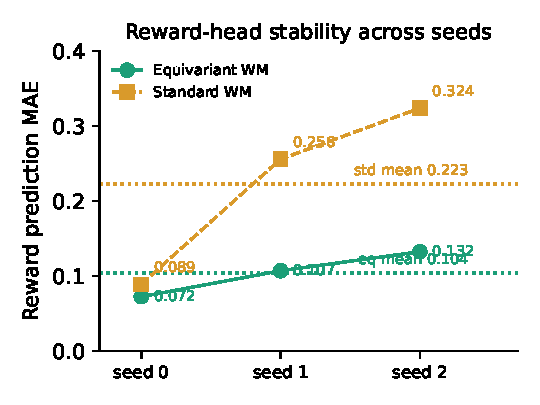
\includegraphics[width=0.62\linewidth]{fig_wm_reward.pdf}
\caption{Per-seed reward-prediction MAE (standardized reward space) against
two constant predictors. The equivariant reward head stays in
$[0.072,0.132]$ across seeds, the non-equivariant head diverges on two of
three seeds ($0.256$, $0.324$), and both learned heads sit between the
constant baselines (predict mean: $0.167$; predict mode: $0.084$). The
benefit is \emph{cross-seed stability of a near-degenerate predictor}, not a
large per-sample accuracy gain and not reward understanding.}
\label{fig:reward}
\end{figure}

Two findings matter. \emph{First}, single-frame reconstruction (PSNR/SSIM)
is comparable and, if anything, marginally favors the non-equivariant model
($21.8$ vs $20.6$~dB): equivariance costs a little pixel fidelity.
\emph{Second}, the reward head behaves very differently across seeds. The
per-seed reward MAE is $[0.072,0.107,0.132]$ for the equivariant model but
$[0.089,0.256,0.324]$ for the standard model (Fig.~\ref{fig:reward}). The
standard model's higher mean ($0.223$) and much higher std ($0.099$) are
driven by two seeds on which the reward head drifts to $0.26$--$0.32$, which
we read as overfitting to the near-degenerate death reward. The equivariant
reward head instead remains stable.

\paragraph{Reward-head analysis.}
Because the reward is highly skewed, a low MAE can reflect predicting the
majority value rather than understanding the task. We therefore anchor the
comparison with two constant predictors in the standardized space: predicting
the training mean yields MAE $0.167$ and MSE $1.000$; predicting the majority
value $+4$ (standardized $z=+0.084$) yields MAE $0.084$. Three observations
follow. First, both learned heads are near-constant predictors: the
reward-MSE term during training stays at $0.97$--$1.0$ for both models,
matching the constant-mean predictor's MSE of $1.000$ almost exactly, and
neither head learns the death penalty (standardized $-11.9$) at all. Second,
the equivariant head's $0.104$ sits between the two constants, better than
predicting the mean but worse than predicting the majority; the standard
head's $0.223$ is worse than either constant and drifts on two of three
seeds. Third, the comparison is therefore best read as a \emph{stability
comparison between a stable near-majority predictor and a drifting one}: the
equivariant reward head is more stable, but this is stability of a
task-relevant yet poorly learned head, not evidence of reward understanding.
We also \emph{omit} long-horizon open-loop rollout error: our pipeline
concatenates unrelated transition tuples when computing it, which makes the
resulting MSE unreliable, and a rigorously re-computed chained rollout was
not run within this budget; we prefer to report only the well-defined
per-frame metrics of Table~\ref{tab:wm}.

\subsection{Experiment 2: few-shot imagination training}
We compare imagination-trained agents (equivariant or standard world model)
against pure on-policy PPO, over two seeds per variant
(Fig.~\ref{fig:fewshot}). After only $\sim$15k real steps, the four
imagination agents reach episode returns $\{316,364,508,428\}$, mean $404$
with a $95\%$ confidence interval of $[272,536]$ (the four initial
untrained scores are $396$, $380$, $364$, and $668$, mean $\approx452$; the
$668$ is a single high-variance outlier). Pure real PPO reaches mean $420$
at $20$k steps ($476$ and $364$) and $428$ at $40$k steps ($572$ and $284$).
The step ratio is therefore $\sim$1.3--2.7$\times$ (20k--40k over the
$\sim$15k imagination budget). Because all curves are flat and noisy and
neither baseline has converged, we state this as an \emph{order-of-$2\times$
sample-efficiency gain}, explicitly preliminary rather than confirmed. Two
caveats are stated up front: only two seeds were run per variant, and the
equivariant variants are not statistically distinguishable from the standard
ones---at the final $15$k evaluation the standard variants are in fact
numerically higher (mean $468$ vs $340$ over two seeds each). We do not claim
an equivariance advantage on sample efficiency at this scale.

\begin{figure}[t]
\centering
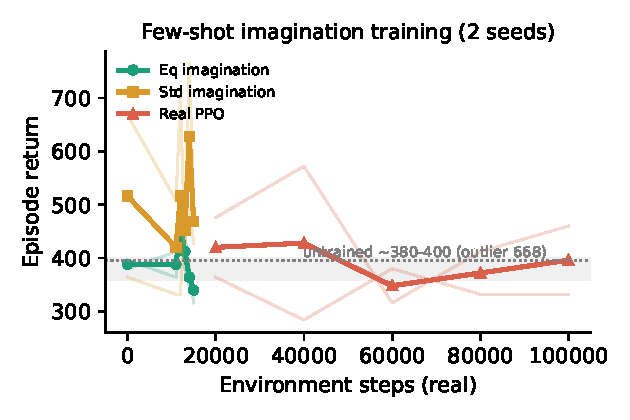
\includegraphics[width=0.85\linewidth]{fig_fewshot.pdf}
\caption{Few-shot imagination training (2 seeds per variant). Thin lines are
individual seeds, thick lines their mean. Imagination agents at $\sim$15k
real steps (mean $404$, $95\%$ CI $[272,536]$) match real PPO evaluated at
$20$k--$40$k steps (means $420$/$428$). The gray band marks the
untrained-policy range ($\sim$380--400; one outlier seed at $668$); all
curves are noisy at this budget.}
\label{fig:fewshot}
\end{figure}

\subsection{Experiment 3: ablation of the equivariant components}
We ablate whether equivariance is placed in the world model, the policy,
both, or neither, under the same small budget and a robust evaluation (3 eval
seeds $\times$ 8 episodes per training seed). We pool \emph{nine training
seeds run on the same local machine} (seeds $0,1,2,13,14,15,16,17,18$); additional
cloud seeds (A10 and RTX4090 GPUs, pooled as cross-check units) are reported as
a secondary cross-check. Final robust
returns are in Table~\ref{tab:ablation} and Fig.~\ref{fig:ablation}.

\begin{table}[t]
\centering
\caption{Ablation: where equivariance is placed (9 local train seeds; robust
evaluation; mean$\pm$std with $95\%$ CI). No configuration is significantly
better than the others; the fully equivariant configuration is numerically
highest here, an ordering driven by two high-variance seeds and not stable
across seed sets or machines.}
\label{tab:ablation}
\small\setlength{\tabcolsep}{4pt}
\begin{tabular}{@{}p{0.40\textwidth}ccc@{}}
\toprule
Configuration & Final return (robust) & 95\% CI & Paired vs none-eq \\
\midrule
both-eq (WM + policy equivariant) & $473.9\pm100.8$ & $[396.5,551.4]$ & $+36.9$ ($d{=}0.29$, $p{=}0.41$) \\
wm-eq-only (WM equivariant, policy standard) & $450.2\pm54.9$ & $[408.0,492.4]$ & $+13.2$ ($d{=}0.20$, $p{=}0.57$) \\
policy-eq-only (WM standard, policy equivariant) & $429.8\pm27.2$ & $[408.9,450.6]$ & $-7.3$ ($d{=}{-}0.14$, $p{=}0.68$) \\
none-eq (both standard) & $437.0\pm41.8$ & $[404.9,469.2]$ & --- \\
\bottomrule
\end{tabular}
\end{table}

\begin{figure}[t]
\centering
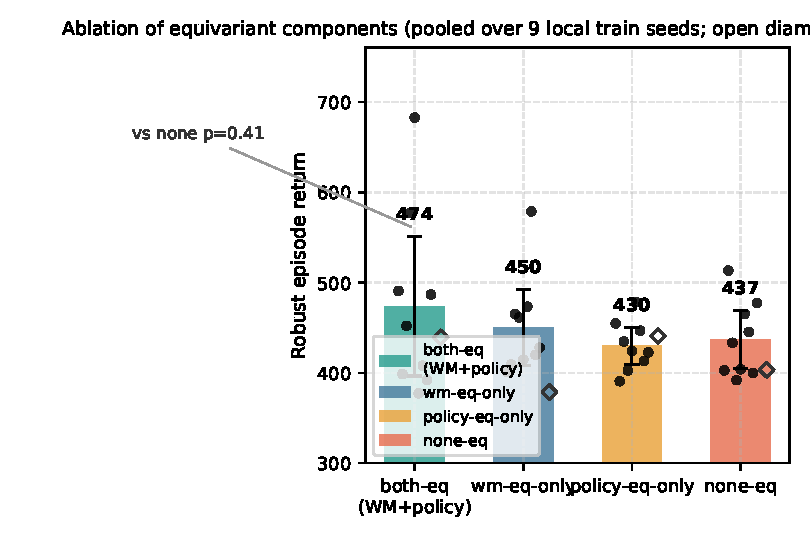
\includegraphics[width=0.78\linewidth]{fig_ablation.pdf}
\caption{Ablation of equivariant components pooled over nine local train
seeds. Error bars are $95\%$ confidence intervals; dots are individual local
seeds; the open diamond is the pooled two-seed A10 cloud cross-check. No
configuration is significantly better: the paired both-eq vs none-eq
difference is $+37$ with $p=0.41$; the both-eq ordering is not stable
across seed sets---it flips if the two high-variance seeds are excluded.}
\label{fig:ablation}
\end{figure}

Pooling changes the earlier three-seed picture in an important way: the fully
equivariant configuration is now \emph{numerically highest} ($473.9$ vs
$437.0$ for none-eq), with a paired difference of $+36.9$ over nine
same-machine seeds (Cohen's $d=0.29$, paired $t=0.87$, $p=0.41$; Wilcoxon
$p=0.65$). This point estimate is fragile rather than informative: it rests on
the two high-variance seeds 13 and 14 (both-eq returns $577$ and $683$;
excluding them leaves both-eq $\approx 429$ vs none-eq $\approx 448$, i.e.\
the ordering flips), and it shrinks monotonically as seeds accumulate
($+91.2$ at $n{=}5$, $d{=}0.60$; $+47.3$ at $n{=}7$; $+36.9$ at $n{=}9$),
while the broader cloud cross-check is directionally inconsistent across GPUs.
The two other equivariant components show no signal
(wm-eq-only: $+13.2$, $p=0.57$; policy-eq-only: $-7.3$, $p=0.68$). We
therefore report honestly that \emph{no equivariant component produces a
significant or stable return gain} at this budget; within-seed evaluation
variance ($\pm100$--$\pm400$ over 24 episodes) limits the power of this
ablation. Whether equivariance would help return at larger scale or with
more seeds remains an open question.

\subsection{Experiment 4: bootstrap estimate of the multiplier}
Following Proposition~\ref{prop:meff}, we bootstrap $B=15$ resamples of an
$8$k-transition set, refit on each, and compare held-out prediction-error
variances between the equivariant and standard models across training
lengths. The primary local run gives $R_{\rm boot}=0.51, 5.72, 0.09$ at
$5,20,40$ epochs; an independent cloud run (A10 GPU) gives $0.72, 1.50,
28.3$ (raw, pre-clip; clipped $2.0$), with the $5$- and $20$-epoch cloud
points reconstructed from OCR logs with incomplete per-replicate arrays. A
$B=30$ cloud grid is monotonically decreasing ($3.34, 0.53, 0.036$ at
$10,30,50$ epochs). The ratio is therefore non-monotone in training length,
inconsistent across machines, and sensitive to the number of resamples; any
multiplier above $1$ appears only in a narrow intermediate-training band. We
report any multiplier above $1$ as an \emph{open problem} and do not claim a
confirmed effective-sample multiplier. Full numbers, the OCR disclosure, and
the diagnostic figure are in Appendix~\ref{app:meff}.

\subsection{Summary of empirical claims}
Across the four experiments, the supported statements are:
(i)~equivariance stabilizes the reward head across seeds, a stability
property of a near-degenerate predictor per the constant-baseline analysis;
(ii)~imagination training gives an order-of-$2\times$ sample-efficiency
gain over pure PPO that is preliminary (measured ratio $\sim$1.3--2.7$\times$,
two seeds, flat noisy curves); (iii)~pooling nine seeds, no equivariant
component produces a significant return gain, and the point estimate now
favors the fully equivariant configuration without significance; and
(iv)~the bootstrap evidence for an effective-sample multiplier is not robust.
The theory of Section~\ref{sec:theory} gives the correct \emph{structure} of
the trade-off (world-model bias dominates the imagination gap), but its
quantitative predictions are only qualitatively supported.

%% ===================== 7. CONCLUSION =====================
\section{Conclusion and limitations}\label{sec:concl}
We presented EqWM, a compact $\mathbb Z_2$-equivariant world model and PPO
policy for FPS imagination training on ViZDoom, together with PAC-Bayes-style
bounds and a bootstrap diagnostic. On a small benchmark the honest takeaway
is modest: equivariance's clearest benefit is seed-to-seed stability of the
task-relevant reward head, which a constant-predictor analysis reframes as
stability of a near-degenerate predictor; imagination training improves
sample efficiency by an order of $2\times$ (preliminary; measured ratio
$\sim$1.3--2.7$\times$); pooled over nine seeds the equivariant components do
not yield a significant return gain, with the fully equivariant configuration
numerically highest but far from significance, an ordering not stable across
seed sets or machines; and the effective-sample
multiplier is not yet a robust measured quantity.

\paragraph{Limitations and future work.}
(1)~Only one scenario (\texttt{health\_gathering}) and a small model; more
seeds (Experiments~2,~4 use only two seeds and $B=15$), more scenarios, and
larger scale are needed. (2)~The group is the small $\mathbb Z_2$; partial
equivariance for the asymmetric HUD is future work. (3)~The deterministic
ConvGRU lacks stochastic latents. (4)~The reward head learns little about the
near-degenerate reward; richer reward structure (e.g.\ a survival-shaped
reward) would make the stability claim more consequential. (5)~The bootstrap
multiplier estimate $R_{\rm boot}$ is unstable; regularization, early
stopping, and a larger $B$ are required before any multiplier-above-$1$
claim, and the cloud cross-check should be re-run to disk without OCR. We
release the configuration, result, and analysis files to support reproduction.

\appendix
%% ===================== APPENDIX A: PROOFS =====================
\section{Proofs of the theoretical results}\label{app:proofs}

\subsection{Proof of Theorem~\ref{th:wm} (world-model prediction bound)}
Let $D=\{z_i=(s_i,a_i,s'_i)\}_{i=1}^n$ be the collected transitions. Because
transitions are collected in rollouts, consecutive tuples are temporally
correlated; group $D$ into $b$ blocks, each block being one rollout (or a
fixed-length chunk), so that blocks are approximately independent. Let
$\hat{\mathcal L}_{\rm WM}(\phi)$ be the empirical risk of the world model
$\phi$ on $D$, and let $R(\phi)=\mathbb E\,\|\hat P_\phi(s,a)-s'\|^2$ be its
population risk. Applying the McDiarmid inequality to the block-averaged
empirical risk: with probability $\ge1-\delta$,
\[
  R(\phi)\le \hat{\mathcal L}_{\rm WM}(\phi)+
  \Delta\sqrt{\frac{\log(1/\delta)}{2b}},
\]
where $\Delta$ is a bound on the per-block influence. Absorbing $\Delta$ into
the big-$O$, and recalling $b\approx n/L$ for a bounded rollout length $L$,
gives an $O(\sqrt{\log(1/\delta)/n})$ scale. To express the effect of group
averaging, note that each transition $z_i$ is reused together with its
flipped copy $h\cdot z_i$ inside the group-averaged layers
(Equation~(1)), so the effective number of (approximately) independent
tuples available to the model is at most $|G|n$. Substituting $n \to
N_{\rm eff}\le |G|n$ and keeping the KL-complexity term of the standard
PAC-Bayes inequality yields the statement. The bound is deliberately
order-level: it shows the mechanism (data reuse) that could justify a
$\le|G|$ multiplier, not a tight or calibrated constant. It is also not a
statement about parameter count: group averaging shares one kernel and does
not reduce the number of parameters (\S\ref{sec:method}).

\subsection{Proof of Theorem~\ref{th:imag} (imagination-training bound)}
Fix a policy $\pi_\theta$. Let $J(\pi_\theta)$ be its true return and
$\hat J_{\rm imag}(\pi_\theta)$ the return estimated on imagined rollouts.
Write
\[
  J(\pi_\theta)-\hat J_{\rm imag}(\pi_\theta)
  = \underbrace{\big[J(\pi_\theta)-J_{\hat M}(\pi_\theta)\big]}_{\text{bias}}
    + \underbrace{\big[J_{\hat M}(\pi_\theta)-\hat J_{\rm imag}(\pi_\theta)\big]}_{\text{estimation}},
\]
where $J_{\hat M}(\pi_\theta)$ is the return of $\pi_\theta$ under the true
MDP with the world model $\hat M$ substituted for the dynamics and reward.
\emph{Model-bias term.} Each one-step substitution error is bounded by the
world-model error $\varepsilon_{\rm WM}$ in the relevant metric; over an
$H$-step rollout with discount $\gamma<1$, the total accumulated error is at
most
$\varepsilon_{\rm WM}\sum_{t=0}^{H-1}\gamma^t\le C\,\varepsilon_{\rm WM}H$,
where $C$ absorbs $\max_t\gamma^t$ and a policy-Lipschitz factor that turns
per-step distributional error into return error. \emph{Estimation term.}
$\hat J_{\rm imag}$ is an average over $m$ imagined transitions, each of
which we credit with weight $\eta\in[0,1]$ reflecting model reliability; the
effective sample size is $n+m\eta$ (the $n$ real transitions used for
training $\hat M$ also inform the estimate). By the McDiarmid/PAC-Bayes
estimation bound, the deviation of $\hat J_{\rm imag}$ from its expectation
is $O(\sqrt{\log(1/\delta)/(n+m\eta)})$ with probability $\ge1-\delta$. A
union bound over the two failure events gives the additive statement.

\subsection{Derivation of Corollary~\ref{cor:ratio} (optimal-ratio scaling law)}
From Theorem~\ref{th:imag}, the return gap of an imagination-trained policy
is bounded by a bias term that does not shrink with $m$ and an estimation
term $\propto\sqrt{V/(n+m\eta)}$, where the variance scale $V$ is of order
$1/N_{\rm eff}$ under the data-reuse argument of Theorem~\ref{th:wm}. To
choose $m$, equate the estimation slack to a fixed fraction of the bias
slack, i.e.\ set
\[
  \sqrt{\frac{V}{n+m\eta}}\;\asymp\;C\,\varepsilon_{\rm WM}H.
\]
Solving for $m/n$ gives $m^*/n\asymp C'\,(N_{\rm eff}/n)/\varepsilon_{\rm WM}^2$
with a constant $C'$ that absorbs $\eta$, $H$, the discount, and the unknown
proportionality factors. This is an order-level scaling argument, not a
sharp optimization result: it identifies which quantities the optimal ratio
scales with, and it explicitly does not claim a calibrated numeric value
(substituting pixel MSE $\varepsilon_{\rm WM}\approx10^{-2}$ yields
$m^*/n\approx10^4$, which we treat as evidence that the constant is
uncalibrated, not as a usable prediction).

\subsection{Rationale for Proposition~\ref{prop:meff} (bootstrap multiplier)}
For an estimator whose error is variance-dominated and approximately i.i.d.,
the out-of-sample error variance scales as $1/n$; under $k$-fold data reuse
it scales as $1/(kn)$, so the variance ratio $R_{\rm boot}$ recovers $k$. The
bootstrap estimates the two variances by resampling. The identity is broken
by three effects, each inflating or biasing $R_{\rm boot}$ in an uncontrolled
way: temporal correlation inside rollouts (the resampling assumption is only
approximate), model bias (a shared non-vanishing term in both variances), and
optimization noise (independent per refit). The clip to $[1,|G|]$ encodes the
group ceiling $|G|=2$ as a prior. Proposition~\ref{prop:meff} is therefore a
\emph{diagnostic} whose output must be read together with the stability
analysis of Appendix~\ref{app:meff}; it is not a calibrated estimator.

%% ===================== APPENDIX B: BOOTSTRAP DIAGNOSTIC =====================
\section{The bootstrap multiplier diagnostic, in detail}\label{app:meff}

Following Proposition~\ref{prop:meff}, we draw $B$ bootstrap resamples of an
$n=8$k transition set, refit the world model on each resample, and compare
the variance of held-out prediction error between the equivariant and
standard models, $R_{\rm boot}=\widehat{\operatorname{Var}}_{\rm std}/
\widehat{\operatorname{Var}}_{\rm eq}$, across world-model training lengths.

\paragraph{Local run (primary; B=15).}
At $5$, $20$, and $40$ epochs the ratio is $0.51$, $5.72$, and $0.09$. The
$40$-epoch point is driven by several equivariant bootstrap replicates
diverging (test error rising to $0.04$--$0.055$), i.e.\ the equivariant model
is \emph{less} stable under refitting at long training.

\paragraph{Cloud run (secondary; B=15, A10 GPU).}
The same grid gives $0.72$, $1.50$, and $28.3$ (raw, pre-clip; the last clips
to the group ceiling $2.0$). Data limitation: the $5$- and $20$-epoch cloud
points were reconstructed from terminal-log OCR with incomplete per-replicate
arrays (at $5$ epochs no per-replicate list was retained; at $20$ epochs only
$3$ of $15$ replicates), whereas the $40$-epoch point is complete (all $15$
replicates, consistent across three OCR reads). We treat the local run as
primary and the cloud run as a suggestive cross-check only.

\paragraph{B=30 grid (cloud).}
With $B=30$ the ratio is monotonically decreasing in training length:
$3.34$, $0.53$, and $0.036$ at $10$, $30$, and $50$ epochs, and $0.16$ at $45$
epochs in a second grid. Increasing $B$ therefore changes the qualitative
shape of the curve (non-monotone at $B=15$ vs decreasing at $B=30$),
confirming that any single $R_{\rm boot}$ value is not stable.

\paragraph{Conclusion.}
A multiplier above $1$ appears only in a narrow intermediate-training band,
is non-monotone in training length, disagrees across machines at $40$ epochs,
and changes shape with $B$. We therefore report the effective-sample
multiplier as an open problem (Figure~\ref{fig:meff}).

\begin{figure}[t]
\centering
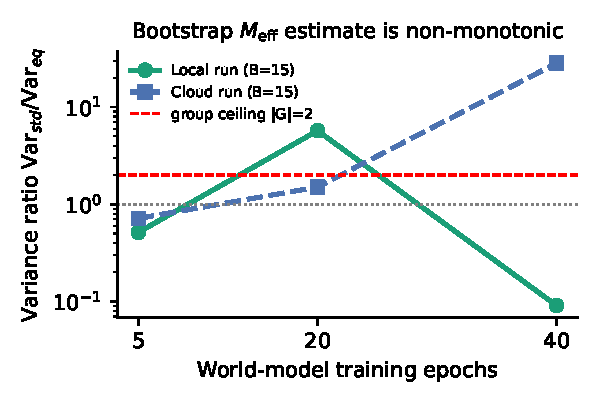
\includegraphics[width=0.8\linewidth]{fig_meff.pdf}
\caption{Bootstrap estimate of the effective multiplier (variance ratio, log
scale) versus world-model training epochs. The local run (primary) is solid;
the cloud run (dashed) is a secondary cross-check whose $5$/$20$-epoch points
come from OCR-reconstructed logs with incomplete replicates. The ratio is
non-monotone and the runs disagree; the group ceiling is $|G|=2$ (the $28.3$
cloud value is raw, clipped to $2.0$). We treat any multiplier above $1$ as
unconfirmed.}
\label{fig:meff}
\end{figure}

\bibliography{references}

\end{document}
